\documentclass[compress,]{beamer}

%loading packages
\usepackage[ngerman]{babel}
\usepackage[T1]{fontenc}
\usepackage[utf8]{inputenc}
\usepackage{tikz}
\usepackage{graphicx}
\usepackage{amsmath}
\usepackage{framed}

%presentation layout
\mode<presentation>{
  \usetheme{Berlin}
  % \usecolortheme{dove}
  \setbeamercolor{structure}{bg=transparent,fg=magenta}
  \setbeamercolor{normal text}{bg=black,fg=white}
  \setbeamercolor{titlepage}{bg=transparent,fg=white}
  \setbeamercolor{titlelike}{bg=transparent,fg=white}
  \setbeamercolor{palette primary}{bg=transparent}
  \setbeamercolor{palette secondary}{bg=transparent, fg=gray}
  \setbeamercolor{palette tertiary}{bg=transparent, fg=magenta}
  \setbeamercolor{palette quarternary}{bg=transparent}
  \setbeamercolor{block title}{bg=magenta,fg=white}
  \setbeamercolor{block body}{bg=white,fg=black}
  \setbeamercovered{transparent}
  \useinnertheme{rectangles}
  %\usefonttheme{serif}
}

% Logo als Wasserzeichen im Hintergrund
\setbeamertemplate{navigation symbols}{}
\setbeamertemplate{background}{
  \tikz[overlay,remember picture]\node[opacity=0.2, at=(current page.south east),anchor=south east,inner sep=4pt]{
    \includegraphics[width=6cm]{images/ZaPFLogo_Berlin_Text.png}
  };
}

% vorgeplaenkel
\title[TU-Konzept]{TU-Konzept}
\author{Ini Physik}
\institute[TU Berlin]

\begin{document}

\subject{Konzept an der TU}
\date{13 Januar 2016}

\begin{frame}
\titlepage
\end{frame}


\frame{\tableofcontents}

\section{Anmeldung}
\begin{frame}{Anmeldung}
  \includegraphics[width=\textwidth]{images/anmeldung.JPG}
\end{frame}

\begin{frame}
  \begin{columns}[onlytextwidth]
    \begin{column}{0.5\textwidth}
      \includegraphics[width=\textwidth]{images/bunker1.JPG}
    \end{column}
    \begin{column}{0.5\textwidth}
      \includegraphics[width=\textwidth]{images/bunker2.JPG}
    \end{column}
  \end{columns}
\end{frame}


\section{Tagungsbüro}
\begin{frame}{EW 109-111}
  \includegraphics[width=\textwidth]{images/tagungsbuero1.JPG}
\end{frame}


\section{Aufenthaltsmöglichkeiten}
\begin{frame}{Foyer im Erdgeschoss und 1. OG}
  \includegraphics<1>[width=\textwidth]{images/foyer1.JPG}
  \includegraphics<2>[width=\textwidth]{images/foyer2.JPG}
  \includegraphics<2>[width=\textwidth]{images/foyer3.JPG}
\end{frame}

\begin{frame}{Campus}
  \includegraphics<1>[width=\textwidth]{images/campus1.JPG}
  \includegraphics<2>[width=\textwidth]{images/campus2.JPG}
\end{frame}


\section{Hörsäle}
\begin{frame}{Hörsaal EW 201}
  \begin{columns}[onlytextwidth]
    \begin{column}{0.5\textwidth}
      \includegraphics[width=\textwidth]{images/DSC_0712.JPG}\\
      \includegraphics[width=\textwidth]{images/DSC_0711.JPG}
    \end{column}
    \begin{column}{0.4\textwidth}
      \begin{block}{Größe}
        286 Sitzplätze
      \end{block}
      \vspace{1cm}
      \begin{block}{Ausstattung}
        PC, Beamer, Funkmikrofon, OH-Projektor
      \end{block}
    \end{column}
  \end{columns}
\end{frame}

\begin{frame}{Hörsäle EW 202 und EW 203}
  \begin{columns}[onlytextwidth]
    \begin{column}{0.5\textwidth}
      \includegraphics[width=\textwidth]{images/DSC_0714.JPG}\\
      \includegraphics[width=\textwidth]{images/DSC_0713.JPG}
    \end{column}
    \begin{column}{0.4\textwidth}
      \begin{block}{Größe}
        EW 202: 127 Sitzplätze\\
        EW 203: 130 Sitzplätze
      \end{block}
      \vspace{1cm}
      \begin{block}{Ausstattung}
        PC, Beamer, Funkmikrofon, OH-Projektor
      \end{block}
    \end{column}
  \end{columns}
\end{frame}


\section{Räume}
\begin{frame}{Seminarräume}
  %hier wollt ich zum Ende egentlich keine Auflistung, sondern Bildersammlung mit entsprechender Bezeichnung
  \begin{columns}[onlytextwidth]
    \begin{column}{0.3\textwidth}
      \begin{itemize}
        \item<1-> \textcolor<1>{magenta}{EW 016}
        \item<2-> \textcolor<2>{magenta}{EW 226}
        \item<3-> \textcolor<3>{magenta}{EW 229}
        \item<4-> \textcolor<4>{magenta}{EW 561}
        \item<5-> \textcolor<5-6>{magenta}{ER 136}
      \end{itemize}
    \end{column}
    \begin{column}{0.7\textwidth}
      % hier wird für jede Raumnummer das entsprechende Bild angezeigt.
      % Beispiel:
      \includegraphics<1>[width=\textwidth]{images/EW016.JPG}
      \includegraphics<2>[width=\textwidth]{images/EW226.JPG}
      \includegraphics<3>[width=\textwidth]{images/EW229.JPG}
      \only<4>{Guckt Euch um!}
      \includegraphics<5>[width=\textwidth]{images/ER136_1.JPG}
      \includegraphics<6>[width=\textwidth]{images/ER136_2.JPG}
    \end{column}
  \end{columns}
\end{frame}

\begin{frame}{Weitere Seminarräume}
  \begin{itemize}
    \item EW 114
    \item EW 431
    \item EW 731
    \item ER 325
  \end{itemize}
\end{frame}

\begin{frame}{Lager- und Gepäckräume}
  \begin{columns}[onlytextwidth]
    \begin{column}{0.3\textwidth}
      \begin{itemize}
        \item<1-> \textcolor<1>{magenta}{EW 182 $\Rightarrow 29,26 \mbox{m}^{2}$}
        \item<2-> EW 184 $\Rightarrow 43,43 \mbox{m}^{2}$
        \item<3-> \textcolor<3>{magenta}{EW 209 $\Rightarrow 33,44 \mbox{m}^{2}$}
        \item<4-> EW 217 $\Rightarrow 51,59 \mbox{m}^{2}$
      \end{itemize}
    \end{column}
    \begin{column}{0.7\textwidth}
      % hier wird für jede Raumnummer das entsprechende Bild angezeigt.
      \includegraphics<1>[width=\textwidth]{images/EW182.JPG}
      \includegraphics<3>[width=\textwidth]{images/EW209.JPG}
      \includegraphics<6>[width=\textwidth]{images/cafeteria.JPG}
    \end{column}
  \end{columns}
  \begin{itemize}
    \item<6-> \textcolor<6>{magenta}{bei der ehemaligen Caféteria gibt es 3 - nach unseren bisherigen Informationen - leere Räume $\Rightarrow\mbox{gesamt ca. 50m}^{2}$}
  \end{itemize}
\end{frame}

\begin{frame}{Rückzugs-/Schlafraum für Orga}
  \begin{columns}[onlytextwidth]
    \begin{column}{0.5\textwidth}
      \begin{itemize}
        \item<1-> GRK-Lounge
      \end{itemize}
    \end{column}
    \begin{column}{0.5\textwidth}
      % hier wird für jede Raumnummer das entsprechende Bild angezeigt.
    \end{column}
  \end{columns}
\end{frame}

\begin{frame}{Weitere Räume, deren Endnutzung noch nicht feststeht}
  \begin{itemize}
    \item PL-Tutor*innenraum
    \item GP-Tutor*innenraum
    \item Atomic und Ini
    \item PC-Pool
    \item MuLF
  \end{itemize}
\end{frame}

\section{Schlafen}
\begin{frame}{Schlafen}
  \begin{columns}[onlytextwidth]
    \begin{column}{0.8\textwidth}
      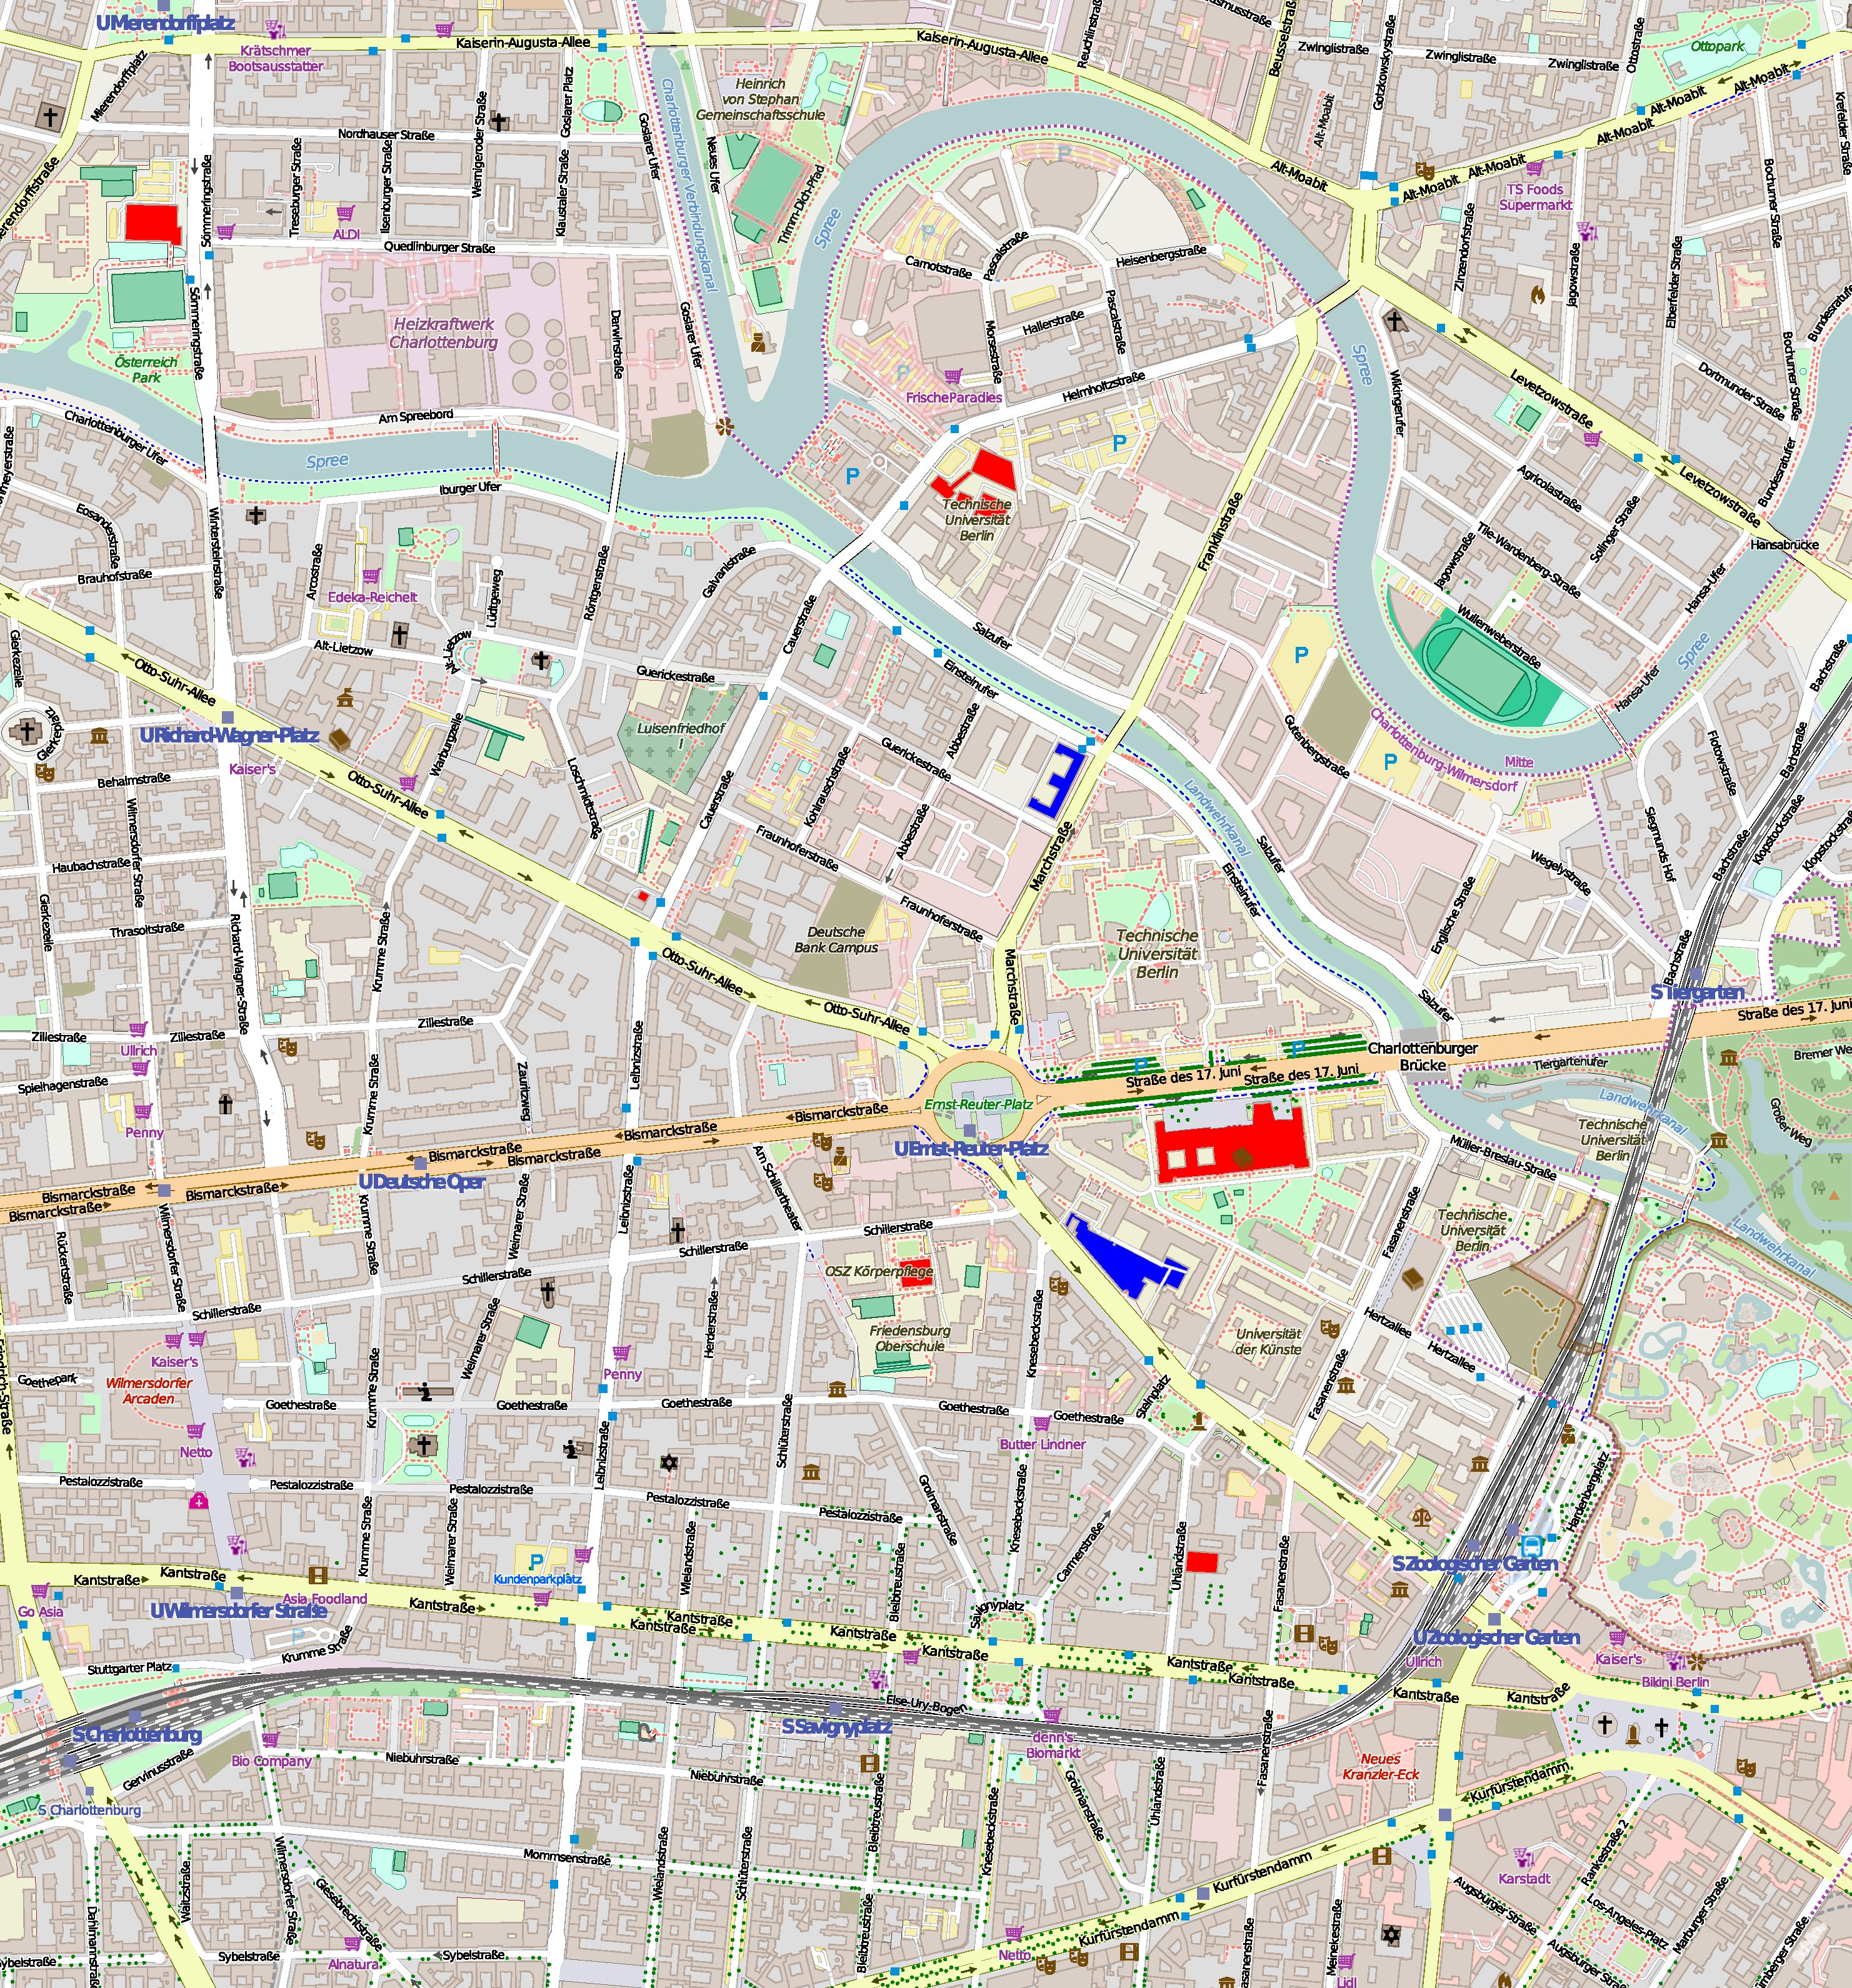
\includegraphics[width=\textwidth,height=\textheight,keepaspectratio]{images/schlafen.pdf}
    \end{column}
    \begin{column}{0.2\textwidth}
      {\color{red} Sporthallen} \\
      {\color{blue} Austragungsorte} \\
      Quelle: Openstreetmap
    \end{column}
  \end{columns}
\end{frame}

\end{document}
